%приложения
%
% листы A1
% Акт об отсутствии заимствований
% Рецензии
%

\appendix

% команды далее необходимы для того, чтобы нумерация элементов текста в приложениях была корректной.
\renewcommand{\theequation}{\thechapter.\arabic{equation}}
\renewcommand{\thefigure}{\thechapter.\arabic{figure}}
\renewcommand{\thetable}{\thechapter.\arabic{table}}
% -------
\renewcommand{\appendixname}{ПРИЛОЖЕНИЯ}
\def\chaptername{ПРИЛОЖЕНИЕ}
\def\thechapter{\Asbuk{chapter}\unskip}
\renewcommand{\thesection}{\thechapter.\arabic{section}\unskip}
%%%%%%%%%%%%%%%%%%%%%%%%%%%%%%%%%%%%%%%%%%%%%%%%%%%%%%%%%%%%%%%%%%%%%%%%
\addcontentsline{toc}{chapter}{ПРИЛОЖЕНИЯ}
%%%%%%%%%%%%%%%%%%%%%%%%%%%%%%%%%%%%%%%%%%%%%%%%%%%%%%%%%%%%%%%%%%%%%%%%
% ПРИЛОЖЕНИЕ
\fancyhead[C]{\thepage \\ \textbf{\leftmark}}
\fancyfoot[C]{}
%----------------------------------------------------------------
\includepdfset{turn=true,scale=0.85,linktodoc=true,pages=-,pagecommand={\pagestyle{fancy}}}
%----------------------------------------------------------------
\chapter{}\label{apx_a1}

\begin{figure}[!ht]
	\centering
	\def\udoffset{10mm}
	\tikzstyle{ar} = [->, >={Stealth[length=8pt]}]
	\tikzstyle{tx} = [midway,sloped,anchor=center, above]
	\begin{tikzpicture}[node distance=2.8cm, scale=1.4]
		\node[state] (S) [xshift=-10mm] {$S_i, h_i$};
		\node[state] (S0) [left of=S] {$\cdots$};
		\node (Sm1) [left of=S0] {$\cdots$};
		\draw [ar] (Sm1) -- (S0);
		\draw [ar] (S0) -- (S);
		\node[state] (S1) [above right of=S, xshift=5mm] {$S_1$};
		\node[state] (S2) [right of=S, xshift=5mm] {$S_2$};
		\node (S11) [right of=S1, xshift=-5mm] {$\cdots$};
		\node (S12) [right of=S2, xshift=-5mm] {$\cdots$};
		\draw [dashed,ar] (S) -- node [tx] {\small $e_{i1}, b_1=1$} (S1);
		\draw [ar] (S1) -- (S11);
		\draw [dashed,ar] (S) -- node [tx] {\small $e_{i2}, b_2=0$} (S2);
		\draw [ar] (S2) -- (S12);
		\draw [dashed,ar] (S) .. controls +(north:1.25*\udoffset) and +(north:1.25*\udoffset) .. node [tx] {\small $e_{i3}, b_3=0$} (S0);
	\end{tikzpicture}
	\caption{Организация ветвления с помощью функции-селектора $h_i$ из состояния $S_i$, где $\forall D_i\filledemptyspoon S_i\rightrightarrows\{S_j\}_{j=1}^{n}$ и $h_i(D_i)=\mbf{b}=(b_1,b_2,b_3,\ldots,b_n)=(1,0,0,\ldots)$. Очевидно, что для представленной иллюстрации $\hat{E}_i=\{e_{i1}\}$ и переход по ветвям, для которых $b_i=0$, запрещён}
	\label{rndhpcedt.20230201.1}
\end{figure}

\chapter{}\label{apx_a2}
\begin{figure}[h]
    \centering
    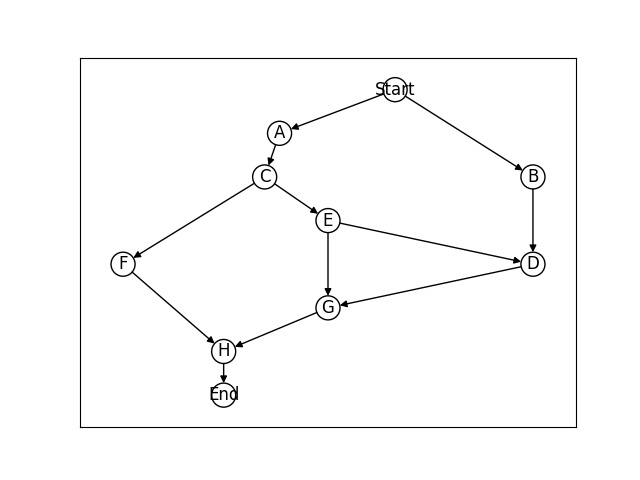
\includegraphics[width=0.55\linewidth]{images/graph.jpg}
    \caption{Пример орграфа без циклов}
    \label{fig:graph}
\end{figure}

\chapter{}\label{apx_a3}
\begin{figure}[h]
    \centering
    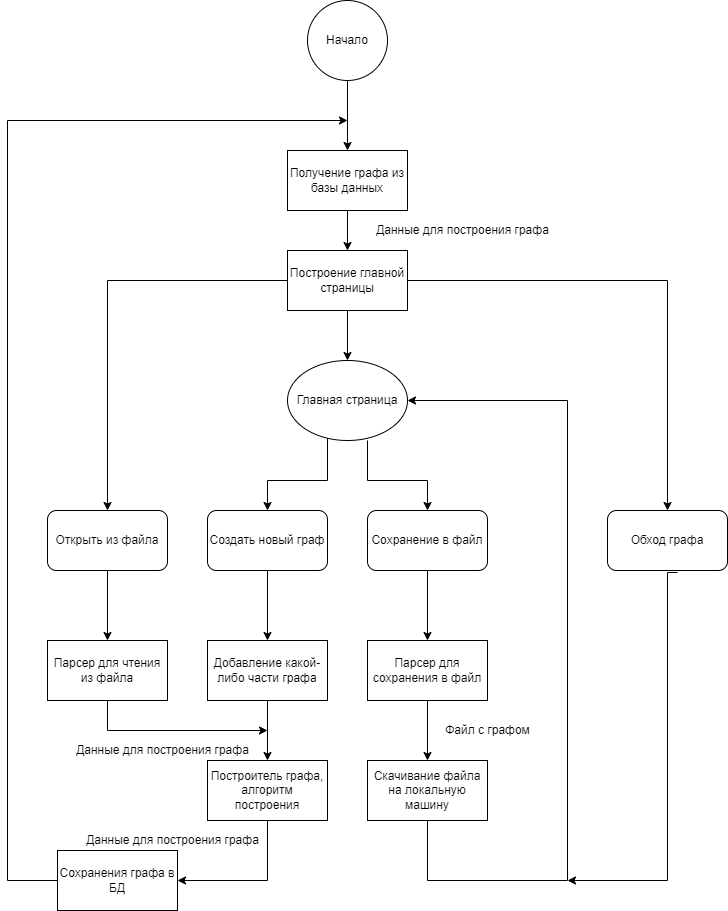
\includegraphics[width=0.7\linewidth]{images/module.png}
    \caption{Схема модулей программы}
    \label{fig:module}
\end{figure} 

\chapter{}\label{apx_a4}
\begin{figure}[!h]
\centerline{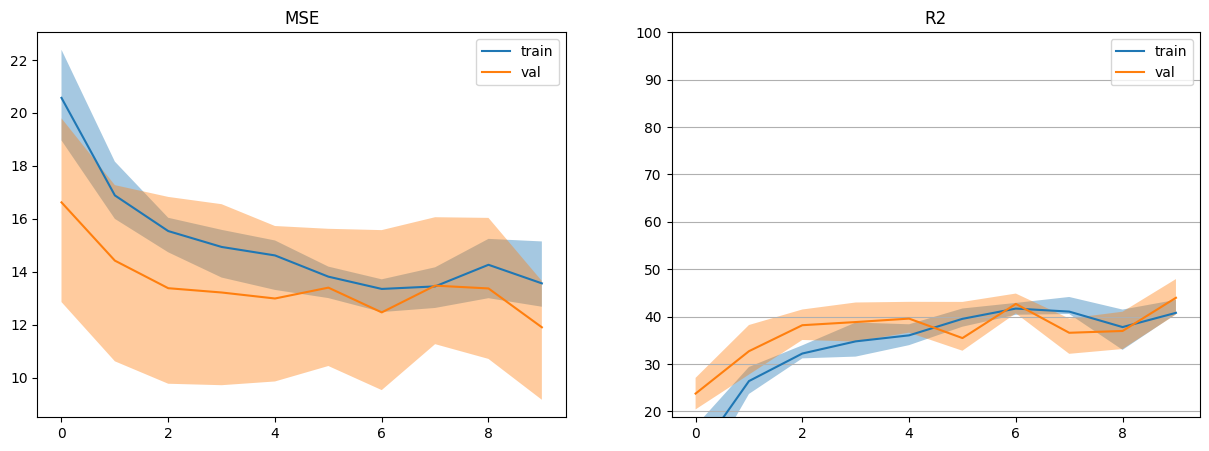
\includegraphics[scale=0.5]{images/1.png}}
\caption{Ориентированный граф созданный с нуля в редакторе}
\label{g1}
\end{figure}

\chapter{}\label{apx_a5}
\begin{figure}[!h]
\centerline{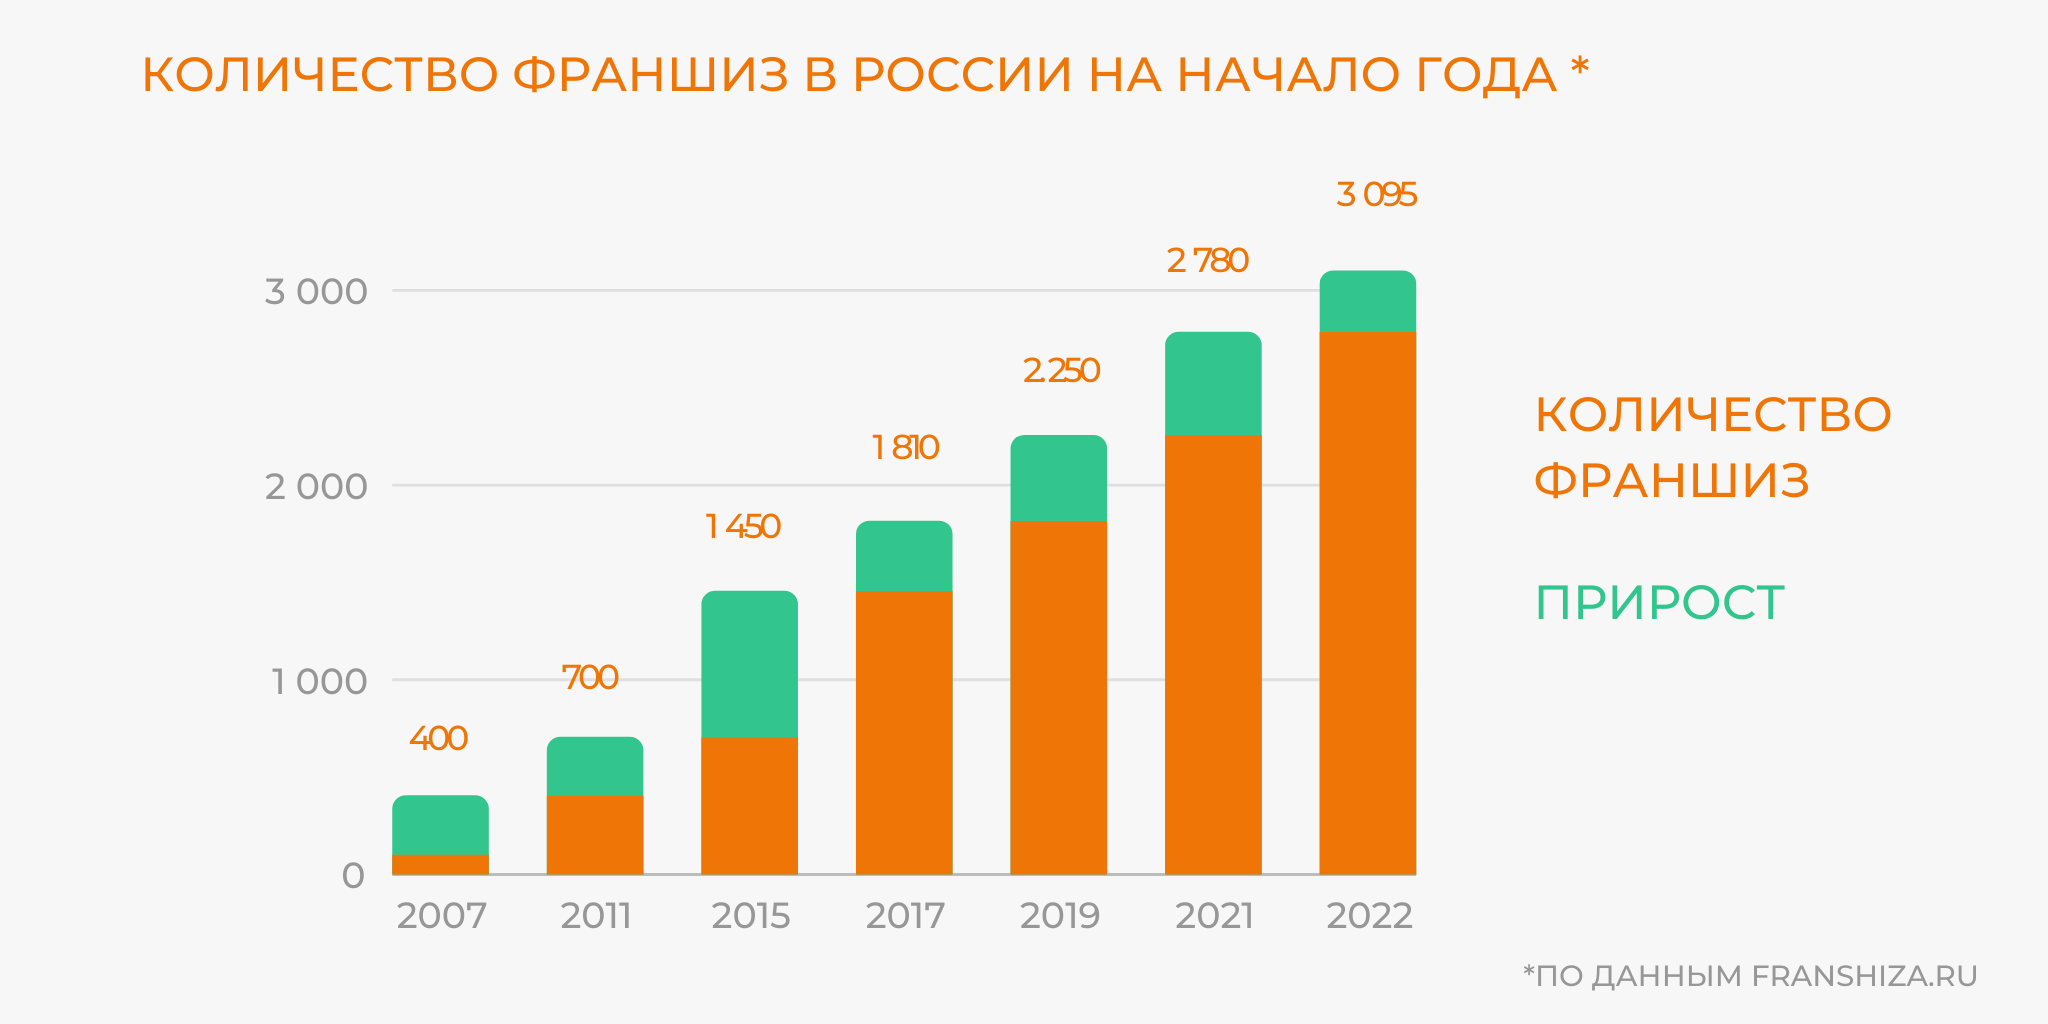
\includegraphics[scale=0.5]{images/2.png}}
\caption{Загруженный в формате aDOT граф}
\label{g2}
\end{figure}

\chapter{}\label{apx_a6}
\begin{figure}[!h]
\centerline{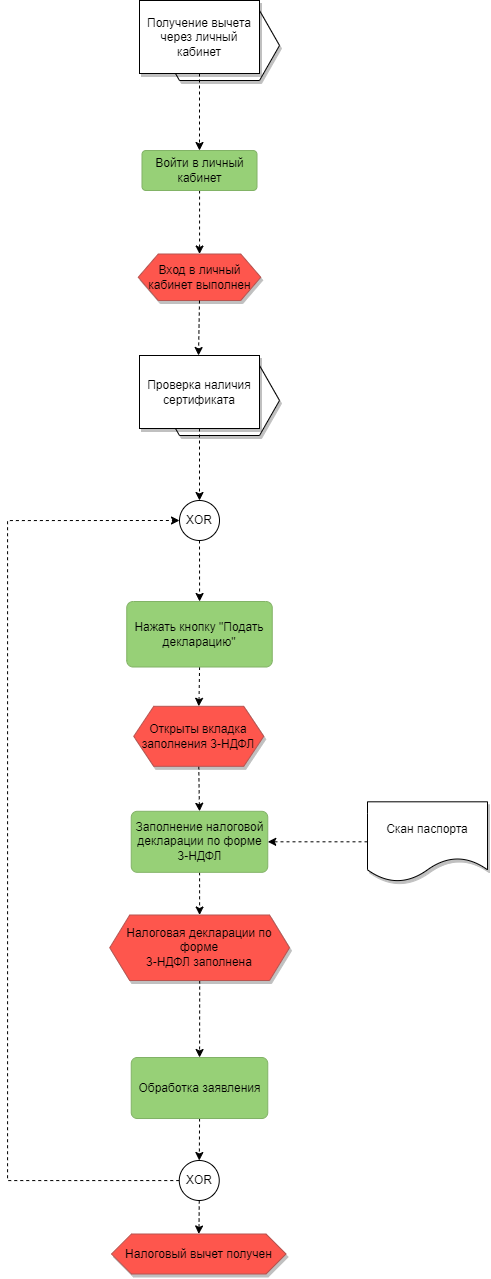
\includegraphics[scale=0.5]{images/4.png}}
\caption{Загруженный в формате aDOT граф}
\label{g3}
\end{figure}
%{\catcode`\_=11
%\newpage
%\includepdf[pagecommand=\label{appx_A1_list1},pages=-]{appendices/appx_A1_list1.pdf}
%}
%
%%{\catcode`\_=11
%%\newpage
%%\includepdf[pagecommand=\label{appx_A1_list1},pages=-]{appendices/appx_A1_list1.pdf}
%%}
%%----------------------------------------------------------------
%\chapter{Акты и рецензии}\label{apx_acts_reviews}
%
%{\catcode`\_=11
%\newpage
%\includepdf[pagecommand=\label{appx_act_plagiat},pages=-]{appendices/appx_act_plagiatpdf}
%}
%
%{\catcode`\_=11
%\newpage
%\includepdf[pagecommand=\label{appx_review_1},pages=-]{appendices/appx_review_1.pdf}
%}

%%%%%%%%%%%%%%%%%%%%%%%%%%%%%%%%%%%%%%%%%%%%%%%%%%%%%%%%%%%%%%%%%%%%%%%%



